\documentclass[a4paper, 11pt]{article}
\usepackage[utf8]{inputenc}
\usepackage{graphicx}
\usepackage{fancyvrb} 
\usepackage{siunitx}
\usepackage[table, xcdraw, svgnames]{xcolor}
\usepackage{listings, lstautogobble}
\usepackage{subfig}

\renewcommand{\figurename}{Figuur}

\setlength{\parskip}{0.5em}

\title{Sensornetwerk Proof of Concept v0.2}
\author{Groep 5}
\date{September 2018}
\pagenumbering{gobble}
\captionsetup[table]{name=\textbf{Tabel}}

\begin{document}

\maketitle
\clearpage
\pagenumbering{arabic}
\clearpage

\section{Inleiding}
Dit document beschrijft de software implementaties van groep 5 voor het vak "Sensornetwerk Ontwerp" aan de Hogeschool van Amsterdam.

Het doel van de opdracht is om een dynamisch netwerk van sensornodes te maken, waarbij in dit document de nadruk ligt op de algemene netwerkstructuur en de implementatie in MCU van de sensornodes. Hiervoor geldt over het algemeen dat het stuk software wat in dit document beschreven wordt gelijk is voor alle sensornodes. Tijdens de ontwikkeling van de individuele sensorimplementaties (vak "Sensormodule Ontwerp") kan de code afhankelijk per node worden aangepast. 

Het doel van dit document is om een 'proof of concept' te geven van de algemene netwerkstuctuur waar de sensornodes tijdens het vak "Sensormodule Ontwerp" gebruik van zullen maken.


\section{Algemene Node Programma}
Zoals besproken in de inleiding van dit document het grootste deel van de programma code voor de node MCU's gelijk. In dit hoofdstuk wordt deze code besproken. 

\subsection{Routing}
Het is belangrijk dat het sensornetwerk dynamisch is. Dit wil zeggen dat het het netwerk waarover de sensordata verstuurd wordt op ieder willekeurig moment kan veranderen. In de praktijk gebeurd dit wanneer de draadloze sensornodes van plaats veranderen of uit gaan. 

Om een 'up to date' beeld te houden van de beschikbare nodes in het netwerk houdt iedere een een routing tabel bij. Deze tabel wordt opgesteld uit berichten die ontvangen worden van de directe buren van de node. In die berichten staat informatie over de directe buren van de nodes die de berichten sturen. 

%%%%%Moet nog aangevuld worden (Zie GLO)%%%%%%%
\subsection{Flowchart}
Om de algemene node-code inzichtelijk te maken is gebruik gemaakt van ene flowchart. In Figuur~\ref{fig:flowchart} is deze flowchart te zien.

\begin{figure}[!h]
	\centering	
	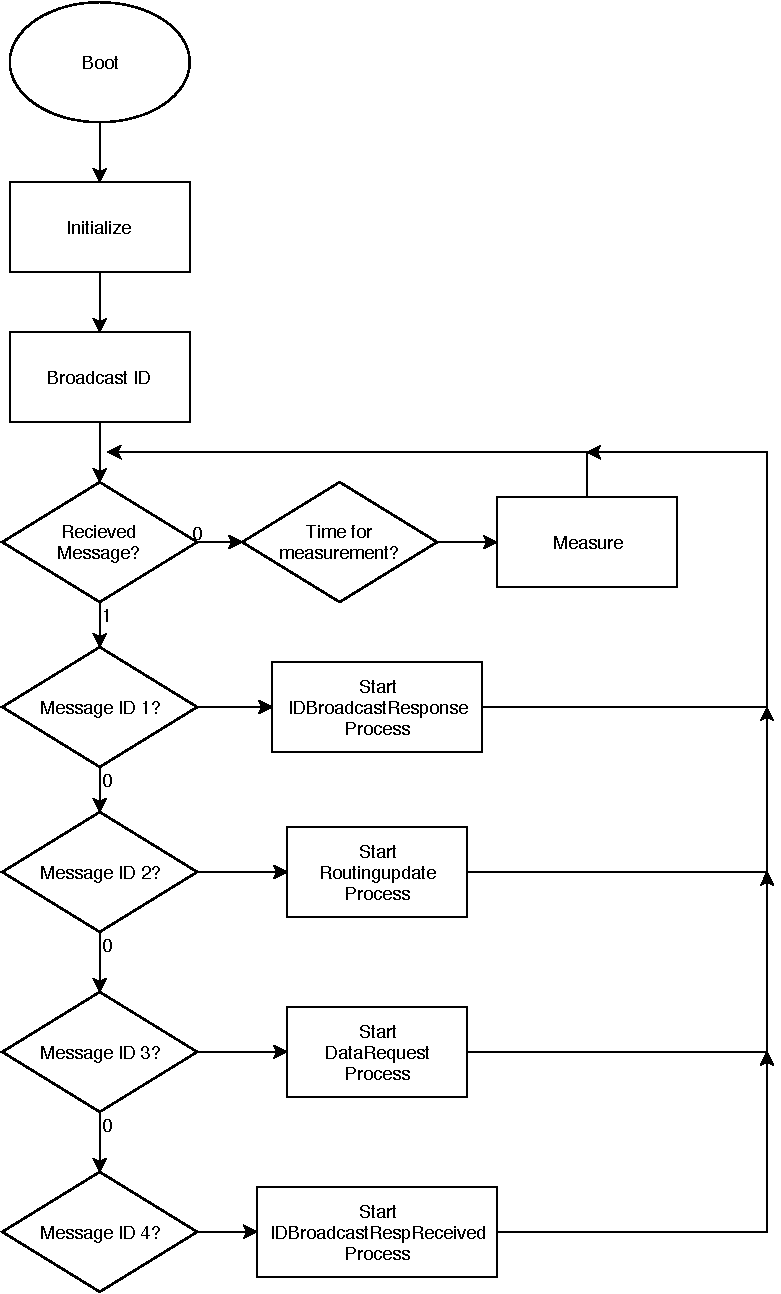
\includegraphics[width=.5\textwidth, keepaspectratio]{media/Pflow.pdf}
    \caption{Nadat de node opgestart wordt (Boot) de MCU geïnitialiseerd in het blok [Initialize]
     \textbf{Figuur dient in deze versie als voorbeeld en zal geupdate worden wanneer het basis ontwerp af is.}}
    \label{fig:flowchart}
\end{figure}
%Zie GLO

\subsection{Statemachine}
Omdat MCU veel aan het wachten is op berichten om deze vervolgens te verwerken is gekozen als implementatie een statemachine te gebruiken. Deze is afgebeeld in Figuur~\ref{fig:Statemachine} 
Statemachine die de verschillende states laat zien waar de Xmega in komt vanaf het opstarten.

\begin{figure}[!ht]
	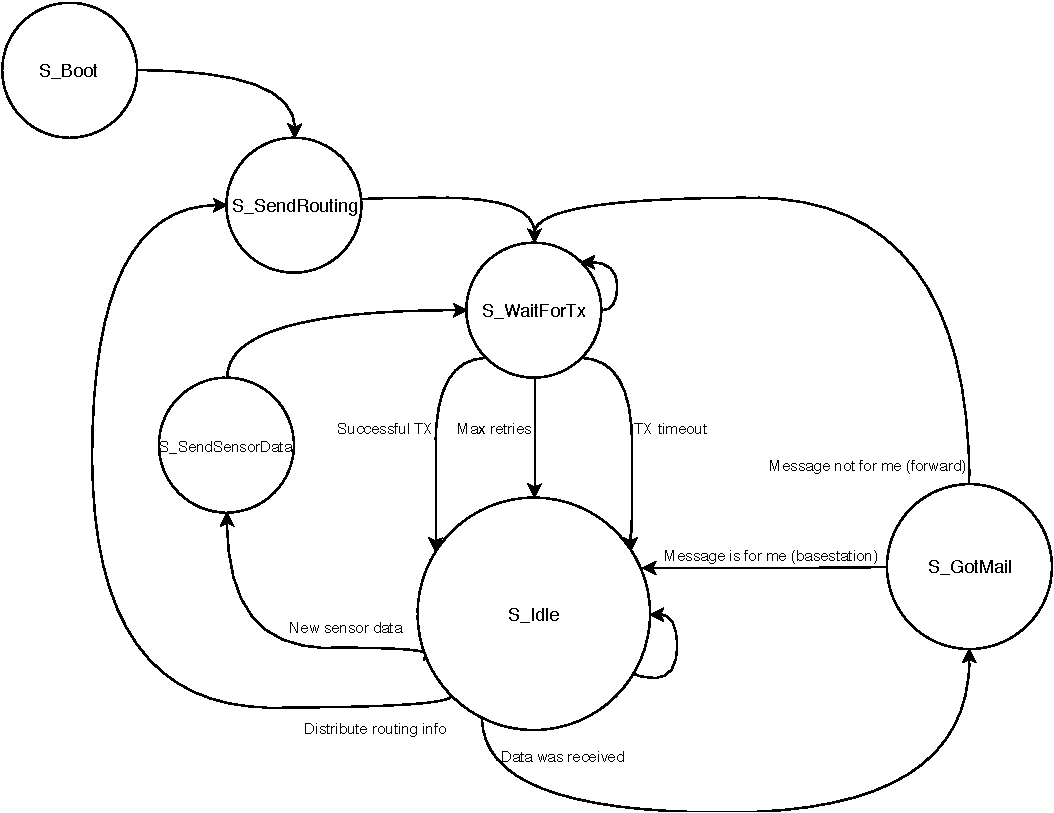
\includegraphics[width=.8\textwidth, keepaspectratio]{media/PState.pdf}
    \caption{ \textbf{Figuur dient in deze versie als voorbeeld en zal geupdate worden wanneer het basis ontwerp af is.}}
    \label{fig:Statemachine}
\end{figure}
%Zie GLO

\section{Basisstation}

\section{ISO groep}
Om te zorgen dat de nodes van de verschillende groepen elkaars datapaketten kunnen interpreteren en doorsturen zijn er afspraken gemaakt tussen de 5 groepen. Elke groep leverde 1 afgevaardigde, de 5 afgevaardigden vormden de ISO groep. De afspraken die de ISO-groep gemaakt heeft zijn opgesteld in\cite{ISO}. 

Naast afspraken over de algemene NRF-instellingen zijn er ook afspraken gemaakt over de berichttypes en de bijbehorende headers.

Bericht headers staan in de onderstaande tabel.
\newpage
\subsection*{Message Types}
\begin{center}
	\begin{table}[!ht]
		\begin{tabular}{|l|l|l|}
			\hline
			\rowcolor[HTML]{EFEFEF} 
			Mask & Description           & Pipe \\ \hline
			0x1  & ID Broadcast          & 0    \\ \hline
			0x2  & Routine Routing Table & 1    \\ \hline
			0x3  & Receive Port Data     & 1    \\ \hline
			0x4  & Broadcast Reply       & 1    \\ \hline
		\end{tabular}
	\end{table}
\end{center}

\section{Netwerk Test}
Om te bewijzen dat het netwerk waar de sensornodes op via zullen opereren werkt, zijn de volgende test uitgevoerd. 
\subsection{Routing Test}
TODO: Beschrijf een test voor het opzetten van een routing tabel met meerdere nodes.
\subsection{Basis Station test}
TODO: Beschrijf een test voor het testen van het Basisstation dat data ontvangt van meerdere nodes. 
\section{Demonstratie proof of concept}
In dit hoofdstuk wordt beschreven hoe de "\textit{proof of concept}" gedemonstreerd wordt. Hierbij zal er onder andere uitleg worden gegeven over de test opstelling, situaties die invloed uitoefenen op het netwerk (zoals het uitvallen van een node) en wat de verwachtingen zijn wanneer dergelijke situaties (niet) optreden. Vervolgens wordt het netwerk onder deze omstandigheden getest en zal het vastgelegd worden d.m.v. datalogs. Op basis van deze datalogs zal uitgelegd worden of het gedrag van het netwerk overeen kwam met onze verwachtingen.
\newpage
\subsection{Testopstelling}
In figuur \ref{testopstelling} is de testopstelling te zien. Hierbij vertegenwoordigen 5 Xmega's de sensor modules en 1 Xmega het basisstation van het netwerk. De Xmega die het basisstation vertegenwoordigd is verbonden met een Raspberry Pi 3b+  waar een Raspberry 7 inch touchscreen display aan verbonden zit. Op dit display word alle ontvangen sensordata per sensor module getoond en een routingtable waarin valt af te lezen welke nodes er zijn gezien in het netwerk en hoeveel hops deze verwijderd zijn van het basisstation.
\begin{figure}[h!]
	\centering
	%\hspace*{-2cm}
	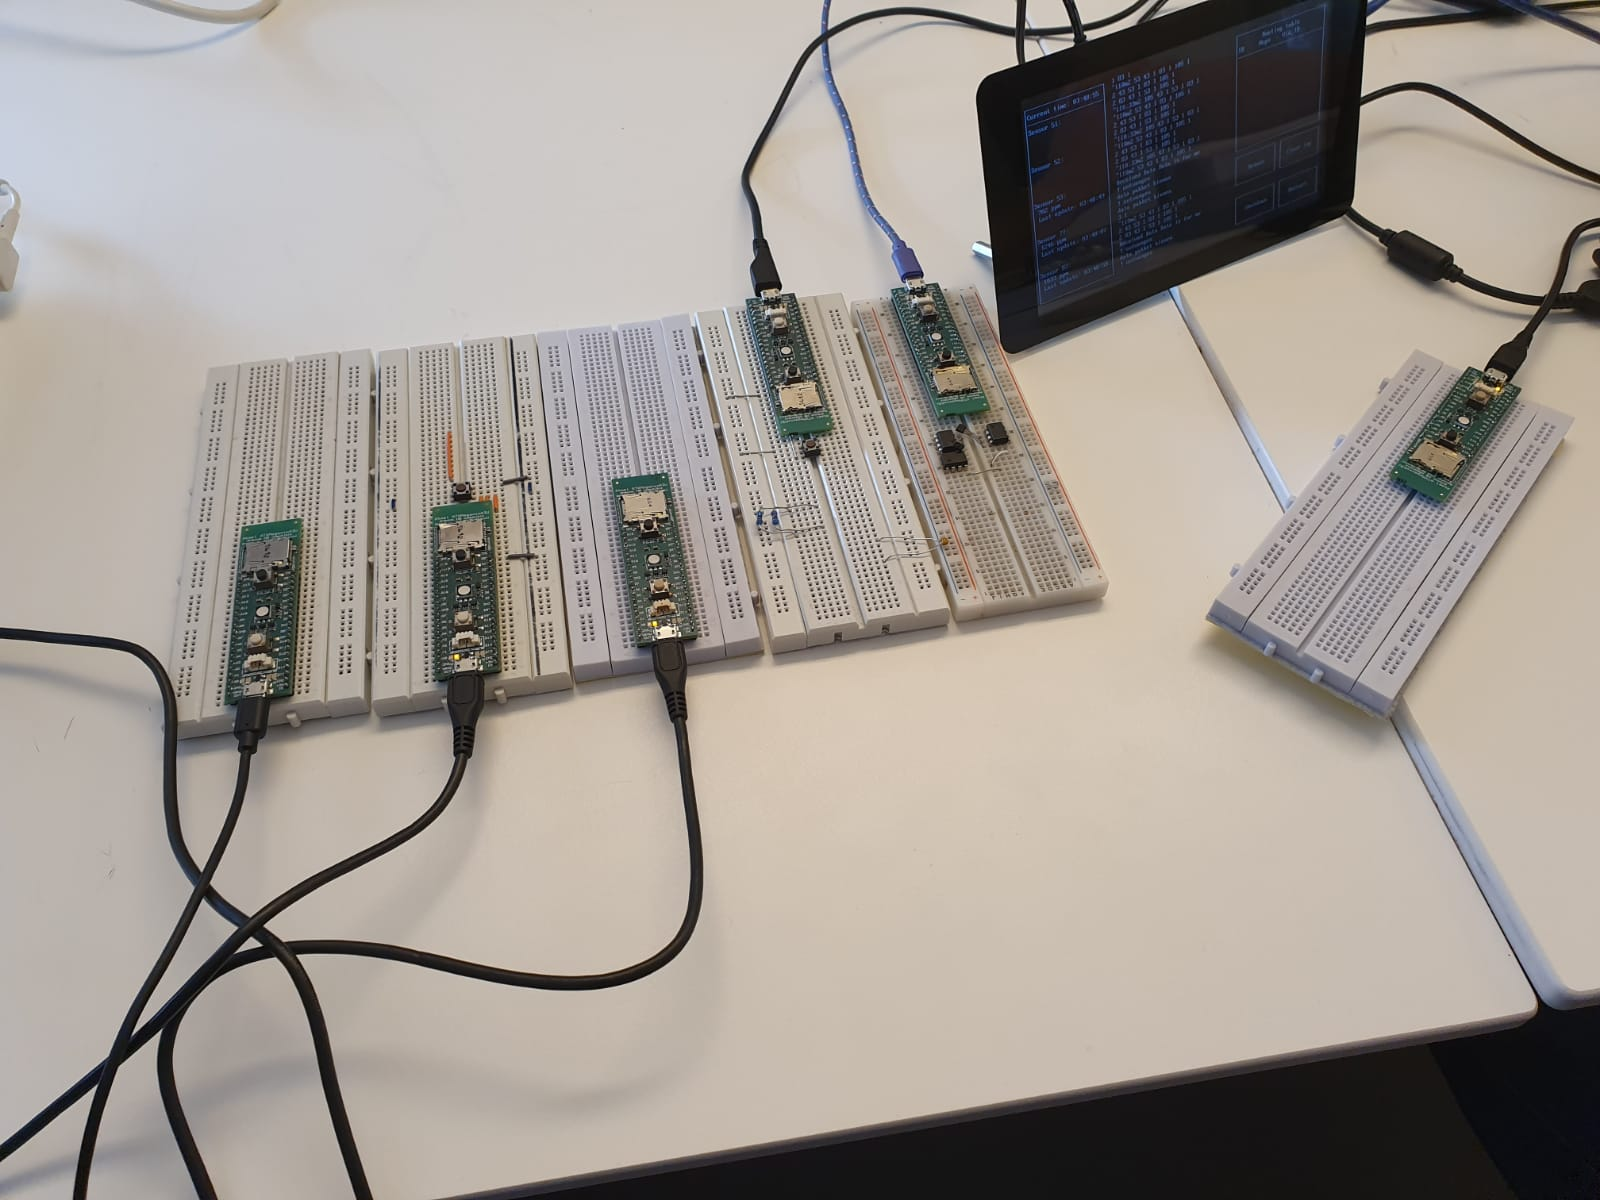
\includegraphics[width=8cm]{media/testOpstellingNetwerk.jpeg}
	\caption{Testopstelling voor de demonstratie van het proof of concept} \label{testopstelling}
\end{figure}

\newpage
\subsection{Situaties die het netwerk veranderen}
In tabel \ref{Situaties} is een overzicht te zien van alle situaties die een belangrijke invloed kunnen hebben op een node. Ook zal er in deze tabel worden omschreven wat de verwachtte reacties van het netwerk zijn op deze situaties.
\begin{table}[ht]
	\centering
	\caption{invloedrijke situaties voor het netwerk en de verwachtte reacties}
	\begin{tabular}{ | m{6cm} | m{6cm}| } 
		\hline
		\textbf{Situatie:} & \textbf{Verwachting:} \\
		\hline
		Sensor module verplaatst zich richting een nieuwe buur & De verplaatste sensor module zal aan de burenlijst worden toegevoegd van de buur waar hij zich naartoe verplaatst heeft
		\\
		\hline
		Sensor module verplaatst zich van een buur af & De verplaatste sensor module zal uit de burenlijst worden verwijderd van de buur waar hij zich vandaan verplaatst heeft en kan eventueel (afhankelijk van de richting en afstand) geen verbinding meer maken met andere sensor modules
		\\
		\hline
		Sensor module valt opeens uit  & De sensor module zal na een bepaalde tijd verwijderd worden uit de burenlijsten en zal in de routingtable bij het basis station als inactief worden gesteld
		\\ 
		\hline
		Sensor module stuurt onzin data over het netwerk & Aangezien het deze berichten waarschijnlijk niet aan de ISO-standaarden voldoen zullen deze niet worden doorgestuurd of opgenomen door het basisstation
		\\ 
		\hline
		Signalen van een sensor module worden opeens geblokkeerd & in principe hetzelfde als wanneer een sensor module uitvalt. Verder zal de sensor module na een bepaalde tijd alle buren uit de burenlijst verwijderen aangezien het ook geen berichten meer ontvangt
		\\ 
		\hline
		Sensor module is niet direct verbonden met het basis station maar wel met andere sensor modules & De sensor module zal proberen via andere sensor modules zijn data bij het basis station terecht te krijgen.
		\\
		\hline
	\end{tabular} 
	\label{Situaties}
\end{table}

\newpage
\bibliographystyle{ieeetr}

\bibliography{POCbronnen} 

\end{document}